\chapter{Basic concepts} % (fold)
\label{cha:basic_concepts}

\section{Web} % (fold)
\label{sec:basic_concepts:web}

\subsection{Contextualization} % (fold)
\label{sub:basic_concepts:web:web:contextualization}

Using concepts from existing hypertext systems, Tim Berners-Lee, computer scientist and at that time employee of CERN, wrote a proposal in March 1989 for what would eventually become the World Wide Web (WWW) \cite{WC2006}.

The World Wide Web is a shared information system operating on top of the Internet \cite{WC2006}. Web browsers retrieve content and display from remote web servers using a stateless and anonymous protocol called HyperText Transfer Protocol (HTTP) \cite{WC2006}. Web pages are written using a simple language called HyperText Markup Language (HTML) \cite{WC2006}. They may be augmented with other technologies such as Cascading Style Sheets (CSS) \cite{CSS2013}, which adds additional layout and style information to the page, and JavaScript (JS) language \cite{International2009}, which allows client-side computation \cite{WC2006}. Client-side refers to operations that are performed by the client in a client-server relationship in a computer network. Typically, a client is a computer application, such as a web browser, that runs on a user's local computer or workstation and connects to a server when necessary. Browsers typically provide other useful features such as bookmarking, history, password management, and accessibility features to accommodate users with disabilities \cite{Grosskurth2005}.

In the beginning of the web, plain text and images were the most advanced features available on the browsers \cite{WC2006}. In 1994, the World Wide Web Consortium (W3C) was founded to promote interoperability among web technologies. Companies behind web browser development, together with the web community, were able to contribute to the W3C specifications \cite{WC2006}. Today's web is a result of the ongoing efforts of an open web community that helps define these technologies and ensure that they're supported in all web browsers \cite{Grosskurth2005}. Those contributions transformed the web in a growing universe of interlinked pages and applications, with videos, photos, interactive content, 3D graphics processed by the Graphics Processing Unit (GPU) \cite{WebGL2013}, and other varieties of features without requiring any third-party plugins installation \cite{Hickson2013}. The significant reuse of open source components among different browsers and the emergence of extensive web standards have caused the browsers to exhibit ``convergent evolution'' \cite{Grosskurth2005}.

The browser main functionality is to present a web resource, by requesting it from the server and displaying it on the browser window \cite{Traffic2013}. There are four major browsers used today: Internet Explorer, Firefox, Safari and Chrome. Currently, the usage share of Firefox, Safari and Chrome together is nearly 60\% \cite{Traffic2013}.

% subsection contextualization (end)

\subsection{Browser architecture} % (fold)
\label{sub:basic_concepts:web:browser_architecture}

For any result or information presented in this work related to the browser environment, three mature browser implementations were selected. For each browser, a conceptual architecture was described based on domain knowledge and available documentation. Firefox version $16.0$, Safari version $6.0.4$ and Chrome version $25.0.1364$ were used to derive the reference architecture because they are mature systems, have reasonably large developer communities and user bases, provide good support for web standards, and are entirely open source \cite{WC2006,Grosskurth2005}. The reference architecture for web browsers is shown in Figure \ref{figure:web_architecture}. It comprises eight major subsystems plus the dependencies between them \cite{Grosskurth2005}:

\begin{enumerate}
  \item User Interface: includes the address bar, back and forward buttons, bookmarking menu and other user interface elements of the browser \cite{Grosskurth2005}.
  \item Browser Engine: an embeddable component that provides a high-level interface for querying and manipulating the Rendering engine \cite{Grosskurth2005,Rocks2013}.
  \item Rendering Engine: performs parsing and layout for HTML documents \cite{Grosskurth2005,Rocks2013}.
  \item Networking Subsystem: used for network calls, like HTTP requests. It has platform independent interface and underneath implementations for each platform \cite{Grosskurth2005,Rocks2013}.
  \item JavaScript Parser: parses and executes the JavaScript \cite{International2009} code \cite{Grosskurth2005}.
  \item XML Parser: parses the HTML markup into a parse tree \cite{Hickson2013}, HTML is rather close to XML \cite{Rocks2013,Hickson2013}.
  \item UI Backend: provides drawing and windowing primitives, user interface widgets, and fonts. Underneath it uses the operating system user interface methods \cite{Grosskurth2005}.
  \item Data Persistence: stores various data associated with the browsing session on disk, including bookmarks, cookies, and cache \cite{Grosskurth2005,Rocks2013}.
\end{enumerate}

\begin{figure}[!htb]
  \centering
  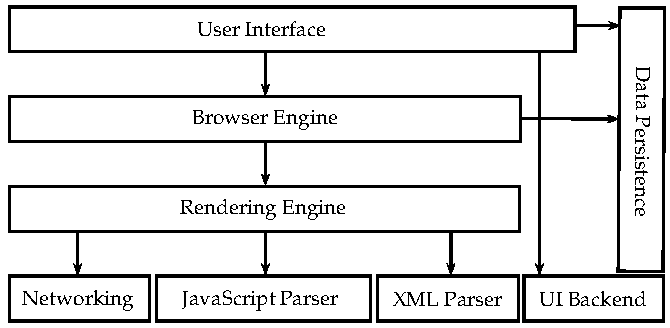
\includegraphics{chapters/basic_concepts/web_architecture.pdf}
  \caption{Reference architecture for web browsers.}
  \label{figure:web_architecture}
\end{figure}

Browser subsystems are swappable \cite{Grosskurth2005} and could vary for each browser vendor, platform or operational system. The browsers mostly differ between different vendors in subsystems (2) the Browser engine, (3) the Rendering engine, and (5) the JavaScript parser  \cite{Firefox2013,Safari2013,WebKit2013,Chrome2010}. In Firefox, subsystems (2) and (3) are known as Gecko \cite{Firefox2013,Gecko2013}, Safari as WebKit \cite{Safari2013,WebKit2013} and Chrome uses a fork of WebKit project called Blink \cite{Chrome2010,Blink2013}. Those browsers subsystems, often called Browser engines, are shown in Figure \ref{figure:web_architecture_engines}.

Another common swappable subsystem is (5) the JavaScript parser. JavaScript \cite{International2009} is a lightweight, interpreted, object-oriented language with first-class functions, most known as the scripting language for Web pages \cite{Gecko2013}. The JavaScript standard is ECMAScript. As of 2013, all modern browsers fully support ECMAScript 5.1. Older browsers support at least ECMAScript 3 \cite{Gecko2013,International2009}.

\begin{figure}[!htb]
  \centering
  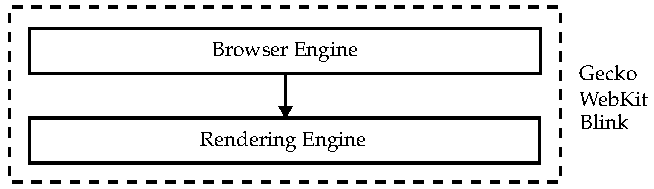
\includegraphics{chapters/basic_concepts/web_architecture_engines.pdf}
  \caption{Reference architecture for browsers engines.}
  \label{figure:web_architecture_engines}
\end{figure}

% subsection browser_architecture (end)

\subsection{Audio and video} % (fold)
\label{sub:basic_concepts:web:audio_and_video}

Audio and video elements were introduced into the browsers by HTML5 specification \cite{Hickson2013}. Audio and video are HTML5 features that attract a lot of attention. Often presented as an alternative to Flash \cite{Flash2013} in the media, the video element has advantages due to its natural integration with the other layers of the web development stack such as CSS \cite{CSS2013} and JavaScript as well as the other HTML elements \cite{WC2006}. The three video formats supported are webm (VP8 Vorbis) \cite{Vorbis2012}, mp4 (H.264 AAC) \cite{AAC2006} and ogv (Theora Vorbis) \cite{Theora2011}. The audio formats available are ogg (Theora Vorbis) and mp4 (H.264 AAC).

Audio and video addition to the browser environment was a good first step for visual tracking applications, on the other hand, the browsers were still not capable of capturing audio and video from the user's microphone and camera, respectively. Audio and video capture has been a limitation of web browsers for a long time \cite{Hickson2013}. For many years the authors had to rely on browser plugins, such as Flash \cite{Flash2013} or Silverlight \cite{Silverlight2013,Rocks2013}. With HTML5, you can now add media to a web page with just a line or two of code \cite{WebKit2013}. Browser audio and video elements \cite{Hickson2013} are shown in Figure \ref{figure:html5_audio_video}.

\begin{figure}[!htb]
  \centering
  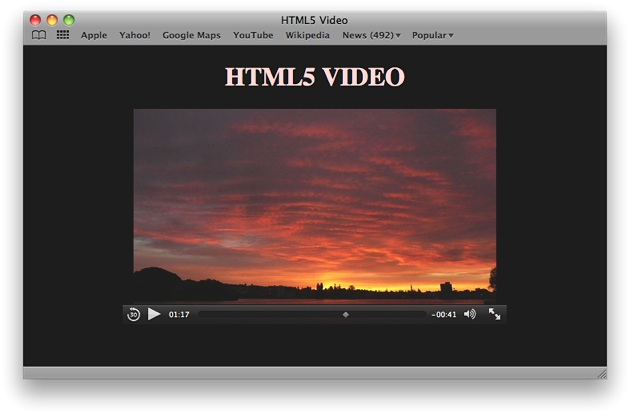
\includegraphics[width=380pt]{chapters/basic_concepts/html5_audio_video.png}
  \caption{Video and audio HTML5 elements \cite{WebKit2013}.}
  \label{figure:html5_audio_video}
\end{figure}

Missing media capturing is no longer a problem for the modern browsers cited in this dissertation \cite{WebRTC2013,Hickson2013}. HTML5 specification has brought a surge of access to device hardware, including Real-time Communication Between Browsers specification (WebRTC) \cite{WebRTC2013} and with Media Capture and Streams specification \cite{MediaCapture2013}. Together, they provide a set of HTML5 and JavaScript APIs \cite{WebRTC2013} that allows local media, including audio and video, to be requested from the user platform \cite{WC2006}. With Media Capture and Streams specification \cite{MediaCapture2013}, the browser can access the microphone and camera input without requiring third-party plugin installation. It's available directly into the browser.

The microphone and camera hardware access can be used in combination with the HTML5 audio and video elements. An example of microphone and camera capturing using a video element is shown on Listing \ref{lst:get_user_media}.

\begin{lstlisting}[language=C++,label={lst:get_user_media},caption=Capture microphone and camera and display using a HTML5 video element.]
<video autoplay></video>
<script>
  var video = document.querySelector('video');
  navigator.getUserMedia({video: true, audio: true}, function(localMediaStream) {
      video.src = window.URL.createObjectURL(localMediaStream);
      video.onloadedmetadata = function(e) { alert('Ready to go.') };
  }, onFail);
</script>
\end{lstlisting}

In Section \ref{sub:basic_concepts:web:canvas_element}, a new HTML5 element called canvas \cite{Canvas2013} is introduced. Through the canvas element video frames can be read, thus providing access to the raw binary data information of each frame. This raw binary data, also known as array of pixels \cite{Gonzalez2007}, is extremely useful for visual tracking applications \cite{Teichrieb2007}. Since the area of study performed on this dissertation is based on visual tracking, from now on, it will focus on camera and video. There are several integration steps required from capturing video to reading the array of pixels. In order to enable the browser to capture the user camera \cite{MediaCapture2013}, stream the information into a video element \cite{Hickson2013}, connect the video to a canvas element, to finally access the array of pixels of each video frame is a long run. The access flow of raw binary data captured from videos on modern browsers is shown in Figure \ref{figure:get_user_media} and comprises four major steps \cite{WebRTC2013,Rocks2013}:

\begin{enumerate}
  \item Hardware access: using HTML5 new Media Capture and Streams specification, the browser microphone and camera hardware is accessed.
  \item Streaming: hardware streams audio and video to the browser UI Elements.
  \item UI Elements: display the video data stream into the browser viewport through a HMTL5 video element \cite{WC2006}.
  \item Raw Binary Data: reads the video frames providing access to the array of pixels through a HTML5 canvas element.
\end{enumerate}

\begin{figure}[!htb]
  \centering
  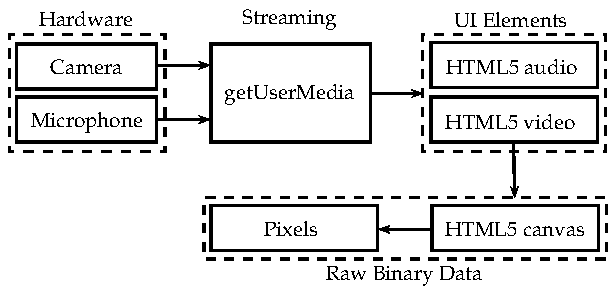
\includegraphics{chapters/basic_concepts/get_user_media.pdf}
  \caption{Access flow of raw binary data captured from videos on modern browsers.}
  \label{figure:get_user_media}
\end{figure}

% subsection audio_and_video (end)

\subsection{Canvas element} % (fold)
\label{sub:basic_concepts:web:canvas_element}

The canvas is an HTML5 element that provides scripts with a resolution-dependent bitmap canvas, which can be used for rendering graphs, game graphics, art, or other visual images on the fly \cite{Canvas2013}.

Authors should not use the canvas element in a document when a more suitable element is available, \eg\ it is inappropriate to use a canvas element to render a page heading. The usage of canvas conveys essentially the same function or purpose as the canvas bitmap. A basic canvas element HTML markup given a width and height in pixels is represented as: <canvas width=``200'' height=``200''></canvas>.

The canvas is a two-dimensional grid that could be described as a simple computer graphics coordinate system \cite{Hartley2004}. Normally one unit in the grid corresponds to one pixel in the canvas. The origin of this grid is positioned at the top left corner coordinate $(0,0)$. All elements are placed relative to this origin. So the position of the top left corner of the blue square shown in Figure \ref{figure:canvas_axis} becomes $x$ pixels from the left and $y$ pixels from the top coordinate $(x,y)$. The canvas coordinate space is shown in Figure \ref{figure:canvas_axis} \cite{MDN2013}.

 \begin{figure}[!htb]
   \centering
   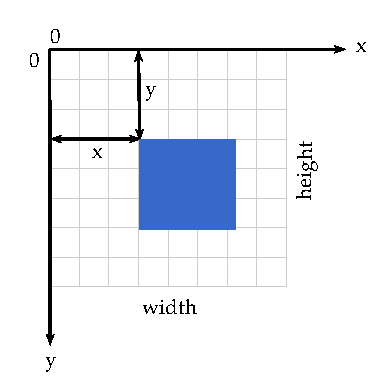
\includegraphics{chapters/basic_concepts/canvas_axis.pdf}
   \caption{The canvas coordinate space.}
   \label{figure:canvas_axis}
 \end{figure}

For each canvas element a ``context'' is available. The canvas context provides the drawing context that can be accessed and JavaScript commands can be invoked to draw or read data \cite{Canvas2013}. Browsers can implement multiple canvas contexts and the different APIs provide the drawing functionality. Most of the major browsers include the 2D canvas context capabilities. Individual vendors have experimented with their own three-dimensional canvas APIs, but none of them have been standardized. The HTML5 specification notes, ``A future version of this specification will probably define a 3D context''. Even though 3D context is not available in most part of the major browsers, three-dimensional applications are already being developed based on the 2D canvas context.

It is mandatory the use of the canvas element to develop visual tracking applications on the web, since it is the only way to read video frames' array of pixels without any plugin in the browser environment. For more information about HTML5 video element see Section \ref{sub:basic_concepts:web:audio_and_video}. Canvas provides APIs to: draw basic shapes, images, videos frames, Bézier \cite{piegl1993fundamental} and quadratic curves \cite{piegl1993fundamental,Hartley2004}; apply transformations, translate, rotate, scale and read the array of pixels information.

% subsection canvas_element (end)

\subsection{JavaScript typed arrays} % (fold)
\label{sub:basic_concepts:web:javascript_typed_arrays}

The JavaScript language \cite{International2009} is intended to be used within some larger environment, be it a browser, server-side scripts, or similar \cite{Grosskurth2005}. JavaScript core language features comprise few major features:

\begin{enumerate}
\item Functions and function scope: function is a subprogram that can be called by external code, functions have a scope they reference for execution.
\item Global objects: refer to objects in the global scope, such as general-purpose constructors (\textit{Array, Boolean, Date} \etc) and typed array constructors (\textit{Float32Array, Int32Array, Uint32Array} \etc).
\item Statements: consist of keywords used with the appropriate syntax (\textit{function, if...else, block, break, const, continue, debugger \etc}).
\item Operators and keywords: arithmetic operators, bitwise operators, assignment operators, comparison operators, logical operators, string operators, member operators and conditional operator \cite{MDN2013}.
\end{enumerate}

As web applications become more and more powerful, adding features such as audio and video manipulation, access to raw data using canvas (Section \ref{sub:basic_concepts:web:audio_and_video}), and so forth, it has become clear that there are times when it would be helpful for JavaScript code to be able to quickly and easily manipulate raw binary data \cite{Canvas2013,TypedArray2013}. In the past, this had to be simulated by treating the raw data as a string and using the \textit{charCodeAt()} method to read the bytes from the data buffer \cite{MDN2013,TypedArray2013}. However, this is slow and error-prone, due to the need for multiple conversions, especially if the binary data is not actually byte-format data, but, for example, 32-bit integers or floats. Superior, and typed data structures were added to JavaScript specification, such as JavaScript-typed arrays \cite{MDN2013,International2009}.

JavaScript-typed arrays provide a mechanism for accessing raw binary data much more efficiently \cite{MDN2013,TypedArray2013}. This dissertation takes advantage of typed arrays in order to achieve acceptable performance and robustness on the web of complex algorithms implementations.

\subsubsection{Typed arrays performance benchmark} % (fold)
\label{subsub:basic_concepts:web:javascript_typed_arrays:typed_arrays_performance_benchmark}

A performance benchmark comparing regular \textit{vs} typed arrays were executed on the three well known open-source browsers, Firefox, Safari and Chrome. The comparison was executed on Mac OS X 10.8.3, 2.6 GHz Intel Core i7 16 GB 1600 MHz RAM. The array types selected were the not strongly typed \textit{Array}; \textit{Float32Array}, which represents an array of 32-bit floating point numbers; and \textit{Uint8Array}, which represents an array of 8-bit unsigned integers \cite{MDN2013}.

In the benchmark, for each array type a read and a write operation was executed $100,000$ times. In order to not compromise benchmark results caused by run-time type conversion \cite{International2009}, the write value used for each array type was proper selected, \eg\ \textit{Number} $1.0$ was used for regular arrays \textit{Array}, \textit{Number} $1.0$ was used for \textit{Float32Array}, and unsigned \textit{Number} $1$ for \textit{Uint8Array}. Regular \textit{vs} typed arrays performance benchmark is shown in Figure \ref{figure:typed_arrays_performance} \cite{TypedArrayPerformance2013}.

As conclusion, typed arrays provides faster read and write operations than regular arrays in JavaScript, \ie\ $7872$ \textit{ops/sec} for unsigned array \textit{vs} $4437$ \textit{ops/sec} for regular arrays in Firefox browser, similar behavior is noticeable on Safari and Chrome, thereby float and unsigned arrays are vastly used on complex algorithms implementations on the web.

\begin{figure}[!htb]
  \begin{tikzpicture}
      \begin{axis}[
          bar width=15pt,
          enlarge x limits=0.25,
          height= 200pt,
          legend cell align=left,
          scaled y ticks=false,
          symbolic x coords={Firefox,Safari,Chrome},
          width=0.85*\textwidth,
          xmajorgrids=true,
          xtick=data,
          ybar=\pgflinewidth,
          ylabel={Operations per second (ops/sec)},
          ylabel style={yshift=10pt},
          ymajorgrids=true,
          ymin=0
      ]
          \addplot[style={wblue, fill=wblue}]
              coordinates {
                (Firefox, 4437)
                (Safari, 2607)
                (Chrome, 679)
              };

          \addplot[style={wred, fill=wred}]
              coordinates {
                (Firefox, 5841)
                (Safari, 2797)
                (Chrome, 1510)
              };

          \addplot[style={worange, fill=worange}]
              coordinates {
                (Firefox, 7872)
                (Safari, 3089)
                (Chrome, 1510)
              };

          \legend{Array,Float32Array,Uint8Array}
      \end{axis}
  \end{tikzpicture}
  \caption{Regular \textit{vs} typed arrays performance benchmark \cite{TypedArrayPerformance2013}.}
  \label{figure:typed_arrays_performance}
\end{figure}

% subsection typed_arrays_performance_benchmark (end)

\subsubsection{What is the relation between typed arrays and canvas?} % (fold)
\label{subsub:basic_concepts:web:javascript_typed_arrays:relation_between_typed_and_canvas}

Reading and writing raw binary data using typed arrays only solves part of the problem of manipulating video and images data. The other missing feature was solved by HTML5 canvas element, which one important feature is to provide access to the array of pixels of those media \cite{Canvas2013,Hickson2013}. The raw binary data is used by visual tracking algorithms. For more information see Section \ref{sub:basic_concepts:web:audio_and_video}.

 Videos and images pixels can be drawn on a canvas bitmap. Canvas raw binary data can be accessed from the canvas JavaScript API as an object of type \textit{ImageData}. Each object has three properties: width, height and data \cite{Canvas2013,MDN2013}. The data property is of type \textit{Uint8ClampedArray} \cite{TypedArray2013} that is a one-dimensional array containing the data in RGBA \cite{Gonzalez2007} order, as integers in the range $0$ to $255$. The \textit{Uint8ClampedArray} interface type is specifically used in the definition of the canvas element's 2D API and its structure is  similar to the previous shown typed array \textit{Uint8Array}.

The \textit{ImageData} data property, or array of pixels, is in row-major order, a multidimensional array in linear memory. For example, consider the $2\times3$ array $\begin{bmatrix}
1 & 2 & 3\\
4 & 5 & 6
\end{bmatrix}$, in row-major order it is laid out contiguously in linear memory as $\begin{bmatrix}
1 & 2 & 3 & 4 & 5 & 6
\end{bmatrix}$. Each array value is represented as integers between $0$ and $255$, where each four-integer group represents the four color channels of one pixel: red, green, blue and alpha (RGBA). While RGBA is sometimes described as a color space, it is actually simply a use of the RGB color model. This array linear typed structure improves read and write performance, since JavaScript is as an interpreted language \cite{MDN2013}, previous knowledge of the type results in faster language execution \cite{TypedArray2013}. An example of the canvas image data array of pixels is shown in Figure \ref{figure:imagedata_array}.

\begin{figure}[!htb]
  \centering
  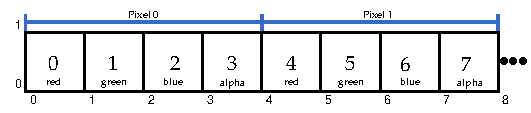
\includegraphics[width=\linewidth]{chapters/basic_concepts/imagedata_array.pdf}
  \caption{The canvas image data array of pixels.}
  \label{figure:imagedata_array}
\end{figure}

% subsection relation_between_typed_and_canvas (end)

% subsection javascript_typed_arrays (end)

% section web (end)

\section{Visual tracking} % (fold)
\label{sec:basic_concepts:visual_tracking}

\subsection{Contextualization} % (fold)
\label{sub:basic_concepts:visual_tracking:contextualization}

Tracking an object in a video sequence means continuously identifying its location when either the object or the camera are moving. There are a variety of approaches, depending on the type of object, the degrees of freedom of the object and the camera, and the target application \cite{Lepetit2005,Teichrieb2007}. Figure \ref{figure:tracking_occlusion} shows a person walking on the street being tracked despite her level of occlusion by another object that is not of interest for the tracking.

\begin{figure}[!htb]
  \centering
  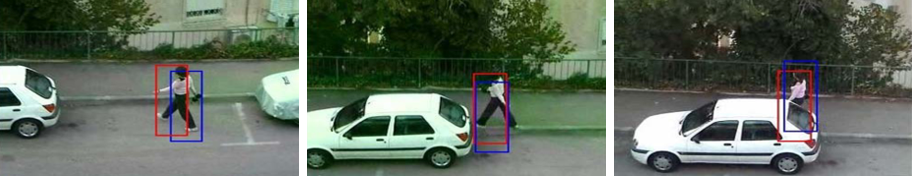
\includegraphics[width=\linewidth]{chapters/basic_concepts/tracking_occlusion.png}
  \caption{Example of an accurate object tracking robust to occlusion \cite{Jia2012}.}
  \label{figure:tracking_occlusion}
\end{figure}

When 2D tracking is used, the goal is to retrieve a 2D transformation from the object projected on the captured image that best represents the motion that occurred. 2D tracking happens on the image space, ignoring the deepness of 3D world \cite{Li2008}. Many models can be applied in order to handle appearance changes due to perspective effects or deformations. The homography is one of the most used transformations regarding 2D tracking of planar objects, since it is generic enough to deal with all possible perspective effects \cite{CMei2008}. This dissertation focuses on the tracking of planar objects since it serves as a basis for more complex tracking approaches (for example, 3D tracking).

In computer vision, general video analysis can be broken down into three different steps: detection of interesting moving objects, frame to frame tracking of those objects and analysis of their tracks to recognize possible behaviors \cite{Yilmaz2006}. Because of such use in computer vision, object tracking is important in the following major areas:

\begin{enumerate}
  \item Augmented Reality (AR) \cite{Azuma1997};
  \item 3D reconstruction \cite{Zhou2008};
  \item Motion-based recognition \cite{Cedras1995};
  \item Automated surveillance \cite{Javed2002};
  \item Video indexing \cite{Javed2002};
  \item Human-computer interaction \cite{Ren2010};
  \item Traffic monitoring \cite{Gloyer1994};
  \item Vehicle navigation \cite{Jia2009}.
\end{enumerate}

Examples of computer vision applications in each of the previously described areas are shown in Figure \ref{figure:cv_applications}. Besides these areas, object tracking algorithms can also be used in AR systems that require real-time registration of the object to be augmented.

\begin{figure}[!htb]
  \centering
  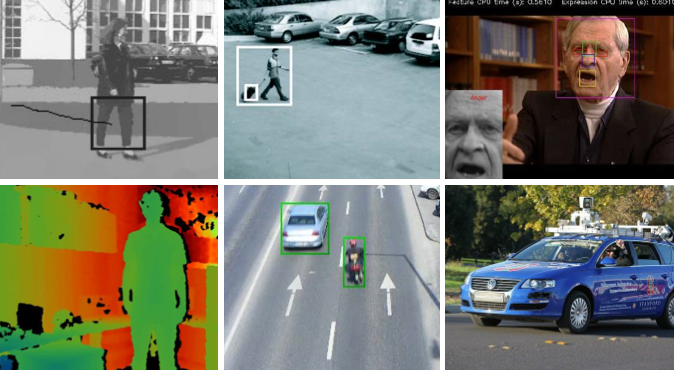
\includegraphics[width=\linewidth]{chapters/basic_concepts/cv_applications.png}
  \caption{Computer vision applications: motion-based recognition (top left) \cite{Cedras1995}; automated surveillance (top center) \cite{Javed2002}; video indexing (top right) \cite{Javed2002}; human-computer interaction (bottom left) \cite{Ren2010}; traffic monitoring (bottom center) \cite{Gloyer1994}; vehicle navigation (bottom right) \cite{Jia2009}.}
  \label{figure:cv_applications}
\end{figure}

Vision has the potential to yield non-invasive, accurate and low-cost solutions for tracking objects. This dissertation introduces a tracking library for the web, that provides visual tracking techniques. Currently, the library provides three main modules, they are: markerless tracking (Section \ref{sec:tracking_library_for_the_web:marker_less_tracking_algorithm}), rapid object detection (Section \ref{sec:tracking_library_for_the_web:rapid_object_detection}) and color tracking (Section \ref{sec:tracking_library_for_the_web:color_tracking_algorithm}).

% subsection contextualization (end)

\subsection{Tracking in augmented reality applications} % (fold)
\label{sub:basic_concepts:visual_tracking:tracking_in_augmented_reality_applications}

Imagine a technology in which you could see more than others see, hear more than others hear, and even touch things that others cannot. A technology able to perceive computational elements and objects within our real world experience that helps us in our daily activities, while interacting almost unconsciously through mere gestures \cite{Krevelen2010,Teichrieb2007}. With such technology, mechanics could see instructions on what to do next when repairing an unknown piece of equipment, surgeons could take advantage of AR while performing surgery on them and we could read reviews for each restaurant in the street we are walking in on the way to work. On the reality-virtuality \textit{continuum} by Milgram and Ki \cite{Mistry2009}, AR is one part of the general area of mixed reality. Both virtual environments (or virtual reality) and augmented virtuality, in which real objects are added to virtual ones, replace the surrounding environment by a virtual one. In contrast, AR provides local virtuality. The reality-virtuality \textit{continuum} is shown in Figure \ref{figure:reality_continuum}.

\begin{figure}[!htb]
  \centering
  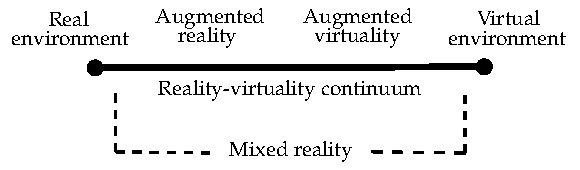
\includegraphics{chapters/basic_concepts/reality_continuum.pdf}
  \caption{Reality-virtuality continuum \cite{Benford1998}.}
  \label{figure:reality_continuum}
\end{figure}

AR applications involve superimposing computer-generated content on real scenes in real-time \cite{Azuma1997}. Tracking is a critical component of most AR applications, since the objects in both real and virtual worlds must be properly aligned with respect to each other in order to preserve the idea of the two worlds coexisting \cite{Zhou2008}.

Traditionally used in AR, vision-based tracking is described as two main steps: extract information from the input video using image processing algorithms and perform the pose estimation itself, or, in other words, find the transformation that best maps the object model from one frame to the next one \cite{Joma2013}.

The information that comes from the input image is basically composed of image features that simplifies extraction from the scene. Both Marker-based AR and Markerless AR \cite{Lima2009a} are based on this principle, with the difference that the first one adds artificial templates, such as special markers that do not originally belong in the scene in order to enable the tracking \cite{Joma2013}. These templates are often called fiducials and they constitute image features easy to extract as well as reliable measurements for the pose estimation \cite{Cho1998,Lepetit2005}. It is therefore much more desirable to rely on naturally present features, such as edges, corners, or texture, those are known as Markerless AR. In this case, the template to be used is the object to be tracked itself, using its natural features.

This dissertation will provide more detail regarding the template-based approaches developed and optimized aiming at web environment.
The template-based tracking techniques do not necessarily rely on local features such as edges or other features, but rather on global region tracking through the use of the whole pattern of the object to be tracked. These methods can be useful in handling more complex objects that are difficult to model using local features due to their repeatability, for example. Such scenarios can be computationally expensive, but in some cases effectively formulated \cite{Yilmaz2006}.

% subsection tracking_in_augmented_reality_applications (end)

\subsection{Which devices could use tracking.js?} % (fold)
\label{sub:basic_concepts:visual_tracking:which_devices_could_use_trackingjs}

Different devices such as mobile phones, notebooks, and even head-worn \cite{Benford1998} (Google Project Glass \cite{Glass2013}), provide an embedded web browser capable to run JavaScript and HTML5. There are several displays devices that could be used on visual tracking or AR applications, Benford \cite{Benford1998}, describes that they could be divided as follows:

\begin{enumerate}
  \item Visual display
    \begin{enumerate}
      \item Video see-through;
      \item Projective;
      \item Monitor.
    \end{enumerate}

  \item Display positioning
    \begin{enumerate}
      \item Head-worn;
      \item Hand-held;
      \item Spatial.
    \end{enumerate}
\end{enumerate}

The possibility to use this work as a cross-platform tracking library is a reality. The browser environment is evolving fast and due to the cross-platform ability, JavaScript is becoming a popular solution for multiple devices and platforms. In a near future, other devices and visual displays may, potentially, embed browser versions, allowing them to benefit from \textit{tracking.js} library.

% subsection which_devices_could_use_tracking_js_ (end)

\subsection{Discussion} % (fold)
\label{sub:basic_concepts:visual_tracking:discussion}

In this dissertation, it was designed and implemented tracking library for the web aiming to provide a common infrastructure to develop applications and to accelerate the use of those techniques on the web in commercial products. Thus, the techniques implemented in this work were chosen aiming to cover common use-cases, such as: facilitate user interaction with the computer trough color tracking (Section \ref{sec:tracking_library_for_the_web:color_tracking_algorithm}); Tracking complex objects in a scene trough markerless tracking (Section \ref{sec:tracking_library_for_the_web:marker_less_tracking_algorithm}); and track humans body parts, \eg\ faces and eyes, trough rapid object detection (Section \ref{sec:tracking_library_for_the_web:rapid_object_detection}).
It runs on native web browsers without requiring third-party plugins installation, therefore any browser-ready device can eventually use the proposed cross-platform code base to develop AR applications. In order to develop for different devices different skills are required, since APIs and programming languages may differ between them \cite{MDN2013,International2009}. In the current day, the most popular devices, such as smart phones, tablets, computers, notebooks and HMD (\ie\ Google Glass \cite{Glass2013}) \cite{Benford1998} are browser-ready \cite{Hickson2013}. They all could benefit from a reusable, cross-platform library for AR applications.

% subsection discussion (end)

% section visual_tracking (end)

% chapter basic_concepts (end)